\section{Estruturais}

\subsection{Adapter}

Quando a interface de uma classe, objeto ou biblioteca não 
é compatível com a interface atual do cliente que deseja 
utilizar essa interface, o padrão Adapter fornece uma 
solução que evita a refatoração e a dependência da interface 
do cliente para a interface desejada.

Existem duas formas de realizar essa adaptação. Um Adapter 
de classe, que só é possível para linguagens que implementam 
herança múltipla, implementa uma classe que herda tanto da 
classe que representa a interface da aplicação quanto da 
classe que representa a interface que deseja ser utilizada. 

\begin{figure}[htb]
	\caption{\label{fig_grafico}Estrutura do Adapter de Classe}
	\begin{center}
	    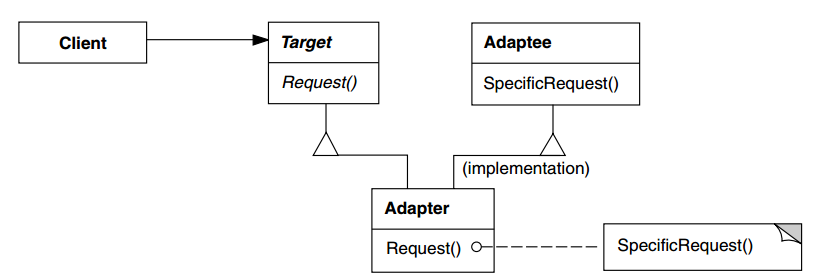
\includegraphics[scale=0.5]{5_padroes-contexto-funcional/5.2_estruturais/5.2.1_adapter/diagram2.png}
	\end{center}
\end{figure}

Já o Adapter de Objeto herda apenas da classe que representa 
a interface da aplicação e reimplementa a operação desejada 
de forma que, após adaptar para a operação para a interface 
desejada, delega a realização da mesma para um objeto que 
implemente essa interface.

\begin{figure}[htb]
	\caption{\label{fig_grafico}Estrutura do Adapter de Objeto}
	\begin{center}
	    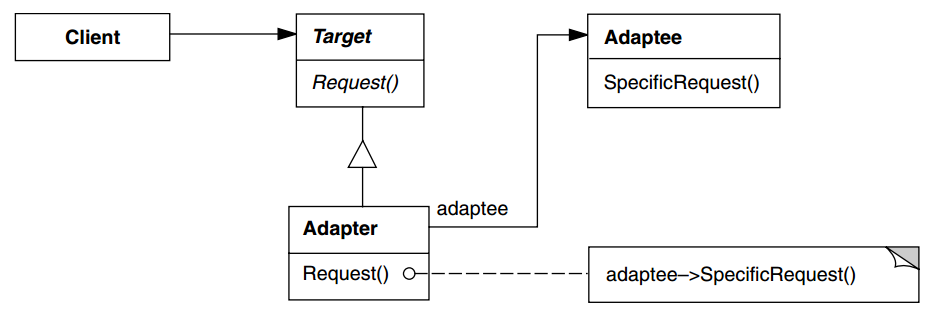
\includegraphics[scale=0.5]{5_padroes-contexto-funcional/5.2_estruturais/5.2.1_adapter/diagram.png}
	\end{center}
\end{figure}

Exemplo Orientado a Objetos:

\begin{lstlisting}[caption={Adapter Orientado a Objetos},label=ooadapter]



\end{lstlisting}

Contexto Funcional:

Existem duas formas simples de implementar um Adapter em uma linguagem 
funcional: usando funções de alta ordem e composição de funções.

Através de funções de alta ordem é possível passar por parâmetro, 
quando necessário, uma função que adapta o valor definido no cliente 
para o valor que precisa ser recebido pela função incompatível. O 
problema dessa abordagem é a necessidade do cliente conhecer a função 
Adapter e a biblioteca.

Já com composição de funções, uma função composta da função Adapter 
e da função incompatível é fornecida para o cliente, que sem precisar 
saber que está usando um Adapter, pode realizar a operação incompatível 
sem problemas.

\begin{lstlisting}[caption={Adapter Funcional},label=fpadapter]
    

    
\end{lstlisting}